\documentclass[aspectratio=169]{beamer}
\usepackage[utf8]{inputenc}
\usepackage{tikz}
\usetikzlibrary{shapes.geometric, arrows, positioning, fit, calc}
\usepackage{graphicx}
\usepackage{booktabs}

% Theme
\usetheme{Madrid}
\usecolortheme{whale}

% Custom Colors
\definecolor{primary}{RGB}{41, 121, 255}
\definecolor{success}{RGB}{0, 200, 83}
\definecolor{danger}{RGB}{255, 82, 82}

% TikZ Styles for Architecture Diagram
\tikzstyle{block} = [rectangle, draw=primary, fill=primary!10, text width=6em, text centered, rounded corners, minimum height=3em, thick]
\tikzstyle{cloud} = [ellipse, draw=gray, fill=gray!10, text width=5em, text centered, minimum height=3em, thick]
\tikzstyle{line} = [draw, -latex', thick]

% Title Page Information
\title[AI Smart Parking]{AI-Powered Smart Parking System}
\subtitle{Reducing CO2 Emissions \& Traffic Congestion using IoT, MARL, GNN \& GRU}
\author[Team]{BTP Project Presentation}
\institute[University]{Department of Computer Science \& Engineering}
\date{\today}

\begin{document}

% Slide 1: Title
\begin{frame}
    \titlepage
\end{frame}

% Slide 2: Outline
\begin{frame}{Outline}
    \tableofcontents
\end{frame}

\section{Problem Statement}
% Slide 3: Problem Statement
\begin{frame}{Problem Statement}
    \begin{itemize}
        \item \textbf{Urban Congestion:} Drivers spend 15-20 minutes searching for parking in urban areas.
        \item \textbf{Environmental Impact:} Idle driving contributes significantly to carbon emissions ($CO_2$) and fuel waste.
        \item \textbf{Inefficient Utilization:} Traditional parking lots lack real-time visibility and dynamic allocation.
        \item \textbf{The Gap:} Existing solutions do not predict future availability or optimize for driver distance.
    \end{itemize}
\end{frame}

\section{System Architecture}
% Slide 4: System Architecture Diagram
\begin{frame}{System Architecture}
    \begin{center}
    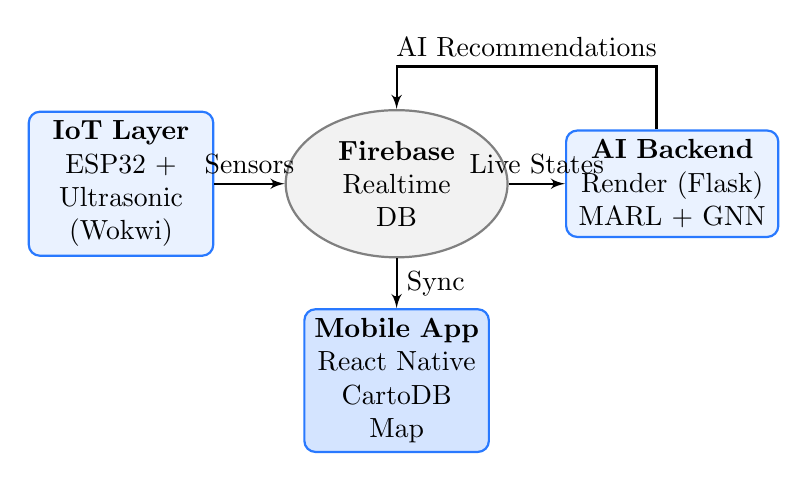
\begin{tikzpicture}[node distance=3.5cm, auto]
        % Nodes
        \node [block] (iot) {\textbf{IoT Layer}\\ESP32 + Ultrasonic (Wokwi)};
        \node [cloud, right of=iot] (db) {\textbf{Firebase}\\Realtime DB};
        \node [block, right of=db, text width=7em] (ai) {\textbf{AI Backend}\\Render (Flask)\\MARL + GNN};
        \node [block, below of=db, node distance=2.5cm, fill=primary!20] (app) {\textbf{Mobile App}\\React Native\\CartoDB Map};

        % Edges
        \path [line] (iot) -- node {Sensors} (db);
        \path [line] (db) -- node {Live States} (ai);
        \path [line] (ai.north) ++(-0.2,0) |- ++(0,0.8) -| node[near start, above] {AI Recommendations} (db.north);
        \path [line] (db) -- node {Sync} (app);
    \end{tikzpicture}
    \end{center}
\end{frame}

\section{Hardware \& IoT}
% Slide 5: Hardware
\begin{frame}{Hardware \& IoT Integration}
    \begin{columns}
        \begin{column}{0.5\textwidth}
            \textbf{Simulation via Wokwi:}
            \begin{itemize}
                \item ESP32 Microcontroller with Wi-Fi module.
                \item 5x Ultrasonic Sensors representing parking slots.
                \item LED indicators (Red = Occupied, Green = Available).
                \item Direct REST API integration with Firebase.
            \end{itemize}
        \end{column}
        \begin{column}{0.5\textwidth}
            \begin{center}
                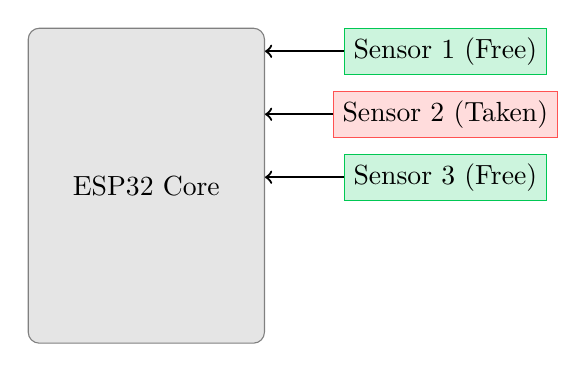
\begin{tikzpicture}[node distance=1.5cm]
                    \node[draw=gray, fill=gray!20, minimum width=3cm, minimum height=4cm, rounded corners] (esp) {ESP32 Core};
                    \node[draw=success, fill=success!20, right=1cm of esp.north east, anchor=north west] (s1) {Sensor 1 (Free)};
                    \node[draw=danger, fill=danger!20, below=0.2cm of s1] (s2) {Sensor 2 (Taken)};
                    \node[draw=success, fill=success!20, below=0.2cm of s2] (s3) {Sensor 3 (Free)};
                    \draw[->, thick] (s1.west) -- (esp.east |- s1.west);
                    \draw[->, thick] (s2.west) -- (esp.east |- s2.west);
                    \draw[->, thick] (s3.west) -- (esp.east |- s3.west);
                \end{tikzpicture}
            \end{center}
        \end{column}
    \end{columns}
\end{frame}

\section{Artificial Intelligence Core}
% Slide 6: AI Core
\begin{frame}{AI Core: MARL, GNN, \& GRU}
    \begin{block}{Graph Neural Networks (GNN)}
        Models the parking lot as a spatial graph to compute actual traversal distances (edges) rather than straight-line (Euclidean) distances.
    \end{block}
    
    \begin{block}{Gated Recurrent Unit (GRU)}
        Analyzes historical occupancy trends to predict if a currently free slot will remain available by the time the driver reaches it.
    \end{block}
    
    \begin{block}{Multi-Agent Reinforcement Learning (MARL)}
        Aggregates GNN distances, GRU predictions, and real-time states to calculate a unified reward score for each slot. Recommends the slot with the highest reward.
    \end{block}
\end{frame}

% Slide 7: Environmental Impact
\begin{frame}{Environmental Impact \& $CO_2$ Savings}
    \begin{columns}
        \begin{column}{0.6\textwidth}
            \begin{itemize}
                \item \textbf{Calculation:} $CO_2 \text{ Saved} = (\text{Time Saved}) \times \text{Emission Rate}$.
                \item Average vehicle emits $\sim 4.6$ metric tons of $CO_2$ per year.
                \item By reducing the search time by just 5 minutes per trip, we save approximately $25g$ of $CO_2$ per parking event.
                \item The React Native mobile app features a gamified dashboard to track total emissions saved by the user.
            \end{itemize}
        \end{column}
        \begin{column}{0.4\textwidth}
            \begin{center}
                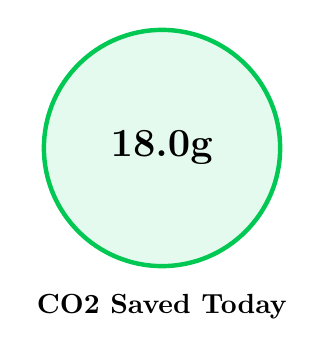
\begin{tikzpicture}
                    \node[circle, draw=success, fill=success!10, minimum size=3cm, ultra thick] (co2) {\Large \textbf{18.0g}};
                    \node[below=0.2cm of co2] {\textbf{CO2 Saved Today}};
                \end{tikzpicture}
            \end{center}
        \end{column}
    \end{columns}
\end{frame}

\section{Results \& Future Scope}
% Slide 8: Results
\begin{frame}{Implementation Results}
    \begin{itemize}
        \item \textbf{Ultra-Low Latency:} End-to-end sync (Sensor $\rightarrow$ AI $\rightarrow$ Map) operates consistently under 3 seconds.
        \item \textbf{Dynamic Cartography:} Fully interactive map interface utilizing CartoDB dark tiles to prevent API billing constraints while maintaining a premium UI.
        \item \textbf{Robustness:} Successfully bypasses free-tier cloud limitations using strategic HTTP polling delays.
    \end{itemize}
\end{frame}

% Slide 9: Future Scope
\begin{frame}{Future Scope}
    \begin{itemize}
        \item \textbf{ALPR Integration:} Automatic License Plate Recognition at entry gates for seamless authentication.
        \item \textbf{Digital Payments:} In-app automated billing based on dwell time via UPI/Credit Cards.
        \item \textbf{Municipal Scaling:} Expanding the GNN model to map entire city blocks and divert traffic at a macro level.
    \end{itemize}
\end{frame}

% Slide 10: Conclusion
\begin{frame}
    \begin{center}
        \Huge \textbf{Thank You!}\\
        \vspace{1cm}
        \Large Any Questions?
    \end{center}
\end{frame}

\end{document}
